\documentclass[border=4pt]{standalone}
\usepackage{tikz}
\usetikzlibrary{positioning,arrows.meta,calc,fit,backgrounds,decorations.pathreplacing}
\usepackage{booktabs}
\usepackage{amsmath,amssymb}
\usepackage{array}
\usepackage{colortbl}
\usepackage{xcolor}

\begin{document}
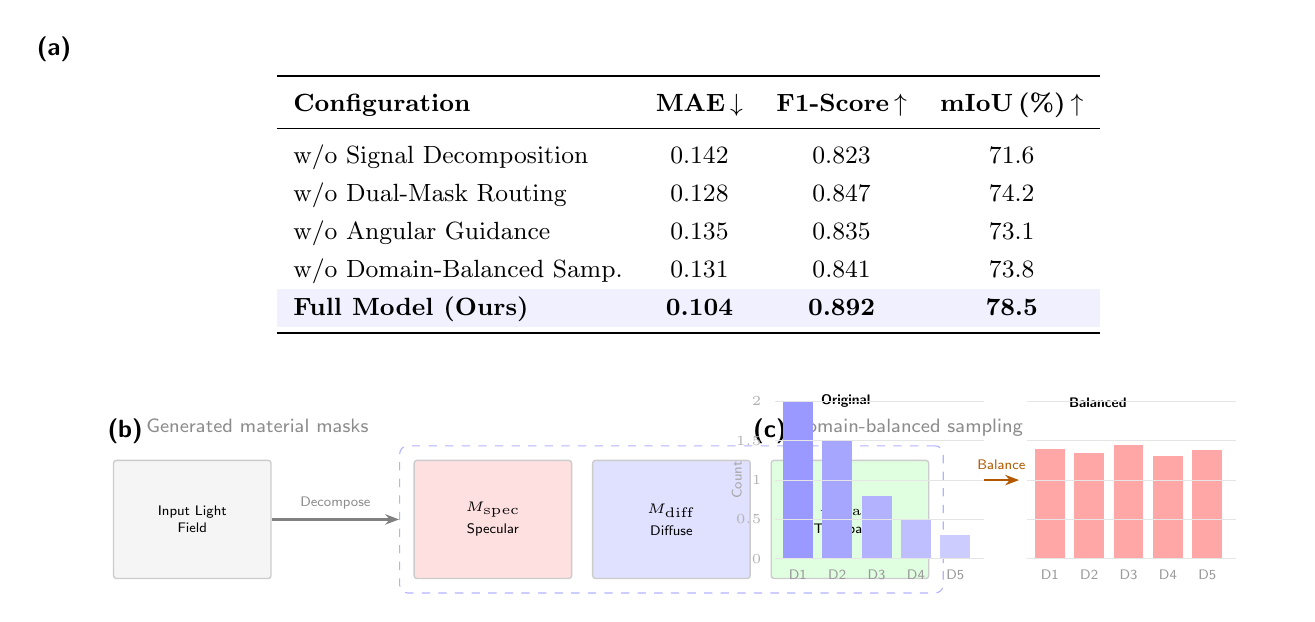
\begin{tikzpicture}[
  imgbox/.style={draw=black!20, rounded corners=1pt,
                 minimum width=2cm, minimum height=1.5cm,
                 inner sep=0pt, font=\sffamily\tiny, align=center,
                 line width=0.5pt},
  arr/.style={-{Stealth[length=5pt]}, thick, color=black!50},
  smallarr/.style={-{Stealth[length=4pt]}, color=black!40},
  plabel/.style={font=\sffamily\bfseries\small},
]

% ===================== Panel (a): Ablation Table =====================
\node[inner sep=0pt] (table) at (7.8,0) {%
  \begin{minipage}{15.2cm}
    \centering\small
    \renewcommand{\arraystretch}{1.25}
    \begin{tabular}{l c c c}
    \toprule
    \textbf{Configuration} & \textbf{MAE\,$\downarrow$} & \textbf{F1-Score\,$\uparrow$} & \textbf{mIoU\,(\%)\,$\uparrow$} \\
    \midrule
    w/o Signal Decomposition     & 0.142 & 0.823 & 71.6 \\
    w/o Dual-Mask Routing        & 0.128 & 0.847 & 74.2 \\
    w/o Angular Guidance         & 0.135 & 0.835 & 73.1 \\
    w/o Domain-Balanced Samp.    & 0.131 & 0.841 & 73.8 \\
    \rowcolor{blue!6}
    \textbf{Full Model (Ours)}   & \textbf{0.104} & \textbf{0.892} & \textbf{78.5} \\
    \bottomrule
    \end{tabular}
  \end{minipage}%
};
\node[plabel, anchor=south east] at ([xshift=-3pt,yshift=1pt]table.north west) {(a)};

% ===================== Panel (b): Mask Visualization =====================
\coordinate (b_anchor) at (0.3,-2.6);
\node[plabel, anchor=north west] at (b_anchor) {(b)};
\node[font=\sffamily\scriptsize, text=black!45, anchor=north west]
  at ([xshift=14pt]b_anchor) {Generated material masks};

% Input
\node[imgbox, fill=gray!8] (b_input) at (1.5,-4.0) {Input Light\\Field};

% Masks
\node[imgbox, fill=red!12, right=1.8cm of b_input] (b_m1) {$M_{\mathrm{spec}}$\\[2pt]Specular};
\node[imgbox, fill=blue!12, right=0.25cm of b_m1]  (b_m2) {$M_{\mathrm{diff}}$\\[2pt]Diffuse};
\node[imgbox, fill=green!12, right=0.25cm of b_m2] (b_m3) {$M_{\mathrm{trans}}$\\[2pt]Transparent};

% Dashed group around masks
\node[draw=blue!30, dashed, rounded corners=3pt, inner sep=5pt,
      fit=(b_m1)(b_m2)(b_m3)] (mask_group) {};

% Arrow from input to mask group
\draw[arr] (b_input.east) --
  node[above, font=\sffamily\tiny, text=black!45] {Decompose} (mask_group.west);

% ===================== Panel (c): Domain-Balanced Sampling =====================
\coordinate (c_anchor) at (8.5,-2.6);
\node[plabel, anchor=north west] at (c_anchor) {(c)};
\node[font=\sffamily\scriptsize, text=black!45, anchor=north west]
  at ([xshift=14pt]c_anchor) {Domain-balanced sampling};

% --- Before bars ---
\node[font=\sffamily\tiny\bfseries, anchor=south] at (9.8,-2.7) {Original};

% Baseline y
\def\bary{-4.5}
\def\barw{0.38}

% Bars: height, x-offset from 8.9
\fill[blue!40] (9.0,\bary) rectangle ++(\barw,2.0);
\fill[blue!35] (9.5,\bary) rectangle ++(\barw,1.5);
\fill[blue!30] (10.0,\bary) rectangle ++(\barw,0.8);
\fill[blue!25] (10.5,\bary) rectangle ++(\barw,0.5);
\fill[blue!20] (11.0,\bary) rectangle ++(\barw,0.3);

% Domain labels under before-bars
\foreach \i/\lbl in {0/D1,1/D2,2/D3,3/D4,4/D5} {
  \node[font=\sffamily\tiny, text=black!40] at (9.19+\i*0.5,\bary-0.2) {\lbl};
}

% Arrow between groups
\draw[-{Stealth[length=5pt]}, thick, color=orange!70!black]
  (11.55,-3.5) -- node[above, font=\sffamily\tiny] {Balance} (12.0,-3.5);

% --- After bars ---
\node[font=\sffamily\tiny\bfseries, anchor=south] at (13.0,-2.7) {Balanced};

\fill[red!35] (12.2,\bary) rectangle ++(\barw,1.4);
\fill[red!35] (12.7,\bary) rectangle ++(\barw,1.35);
\fill[red!35] (13.2,\bary) rectangle ++(\barw,1.45);
\fill[red!35] (13.7,\bary) rectangle ++(\barw,1.3);
\fill[red!35] (14.2,\bary) rectangle ++(\barw,1.38);

% Domain labels under after-bars
\foreach \i/\lbl in {0/D1,1/D2,2/D3,3/D4,4/D5} {
  \node[font=\sffamily\tiny, text=black!40] at (12.39+\i*0.5,\bary-0.2) {\lbl};
}

% Baseline lines
\draw[black!20] (8.9,\bary) -- (11.55,\bary);
\draw[black!20] (12.1,\bary) -- (14.75,\bary);

% Y-axis ticks (sample count indication)
\foreach \v/\y in {0/0, 0.5/0.5, 1.0/1.0, 1.5/1.5, 2.0/2.0} {
  \node[font=\sffamily\tiny, text=black!30, anchor=east] at (8.85,\bary+\v) {\pgfmathprintnumber[fixed,precision=1]{\v}};
  \draw[black!10] (8.9,\bary+\v) -- (11.55,\bary+\v);
  \draw[black!10] (12.1,\bary+\v) -- (14.75,\bary+\v);
}

% Sample count label
\node[font=\sffamily\tiny, text=black!35, rotate=90, anchor=south] at (8.6,-3.5) {Count};

\end{tikzpicture}
\end{document}